
\subsubsection{API Gateway trong Microservice (Kong API Gateway)}

API Gateway
được sử dụng
để quản lý
và kiểm soát việc truy cập vào các API.
API Gateway cung cấp một lớp trung gian
giữa client và các dịch vụ.
Có thể nói, API Gateway
là một điểm vào độc lập cho nhiều client của một ứng dụng.
Kong API Gateway
là một trong những API Gateway
mã nguồn mở
phổ biến
có thể quản lý
các API được triển khai ở bất kỳ đâu,
từ cơ sở hạ tầng đơn giản đến môi trường đa đám mây phức tạp.

\begin{figure}[H]
\centering
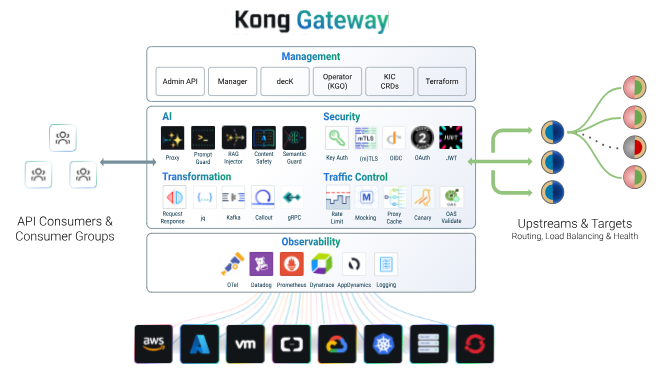
\includegraphics[width=0.95\textwidth]{pictures/kong-gateway-overview.excalidraw.png}
\caption{Sơ đồ tổng quan kiến trúc và luồng hoạt động của Kong API Gateway}
\end{figure}

Cấu trúc dự án Kong API Gateway

\begin{figure}[H]
\centering
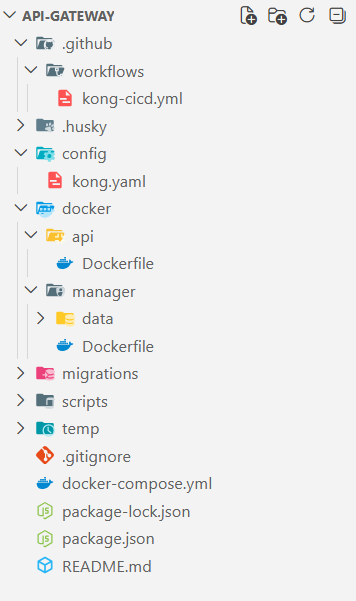
\includegraphics[scale = 0.6]{pictures/kong-api-gateway-project-v2.png}
\caption{Cấu trúc dự án Kong API Gateway}
\end{figure}

Trong
môi trường sản xuất thực tế
gặp nhiều thách thức, khó khăn.
Em sử dụng các plugin của Kong API Gateway như
rate limit giới hạn tốc độ yêu cầu,
bot-detection ngăn chặn các yêu cầu độc hại.

\begin{figure}[H]
\centering
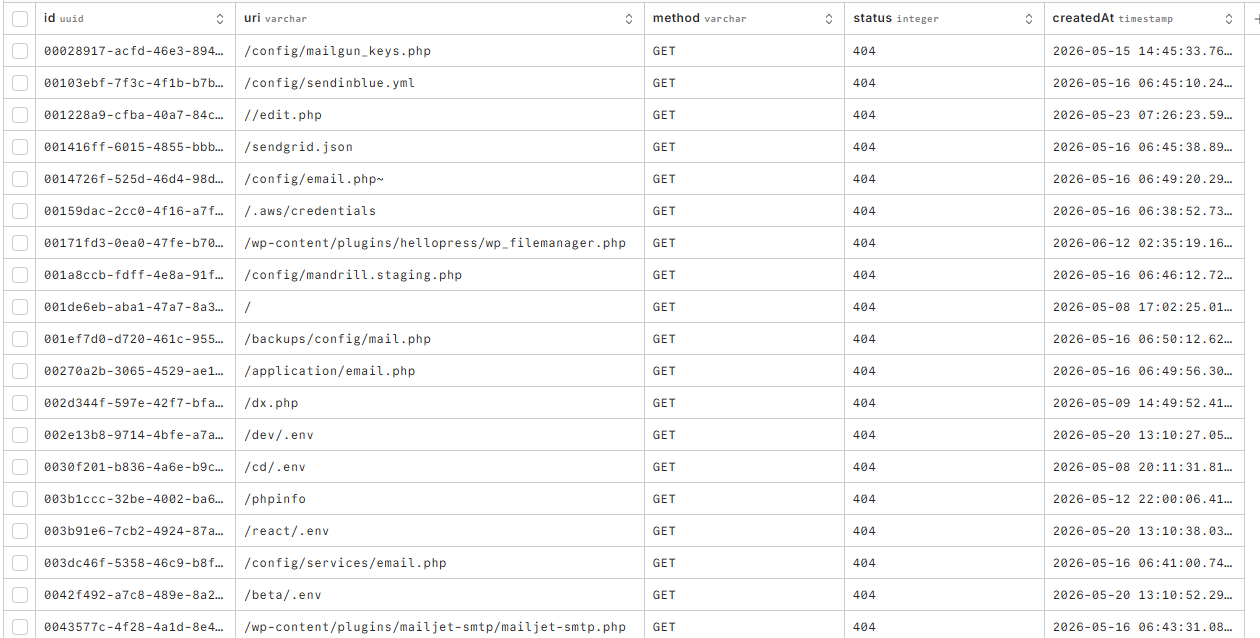
\includegraphics[width=0.95\textwidth]{pictures/kong-api-gateway-env-secret.png}
\caption{Các yêu cầu độc hại dò các bí mật nhạy cảm (404 Not Found)}
\end{figure}

Sơ đồ quản lý Kong API Gateway

\begin{figure}[H]
\centering
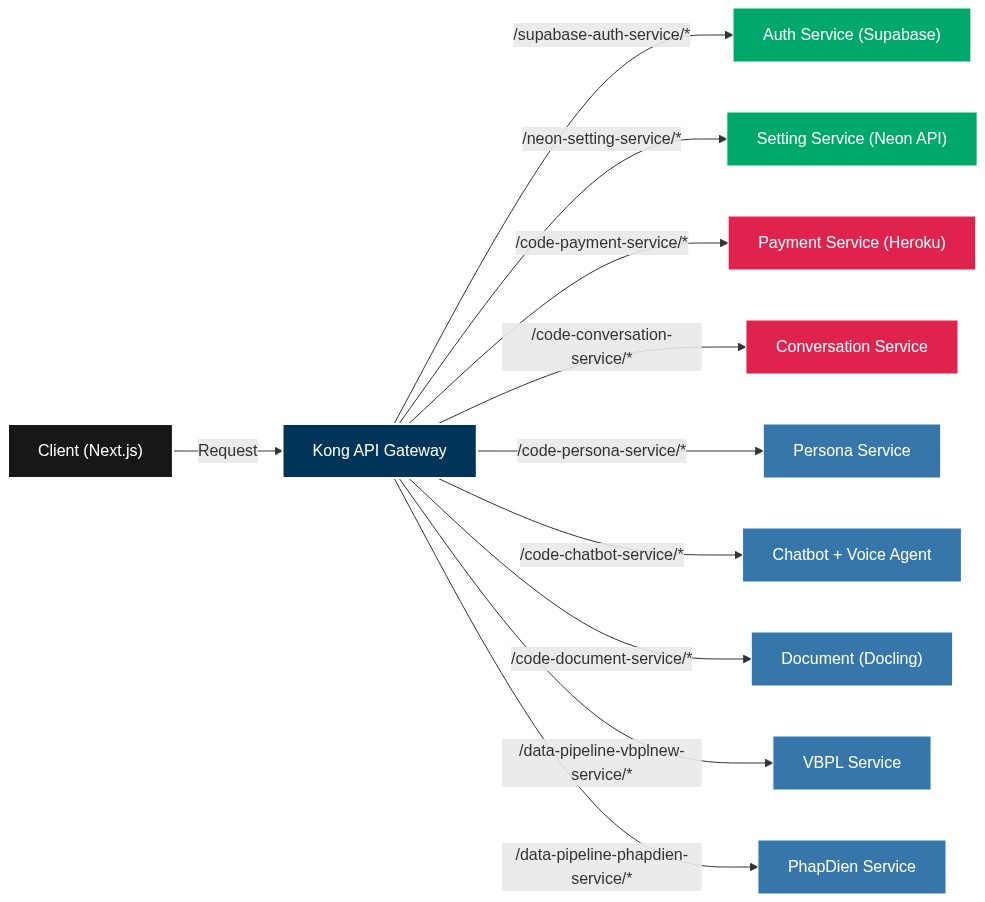
\includegraphics[width=0.95\textwidth]{pictures/kong-api-gateway-router.png}
\caption{Thiết lập định tuyến dịch vụ (Routes) trong Kong API Gateway}
\end{figure}

Có nhiều cách quản lý => ưu điểm của DECK

\begin{figure}[H]
\centering
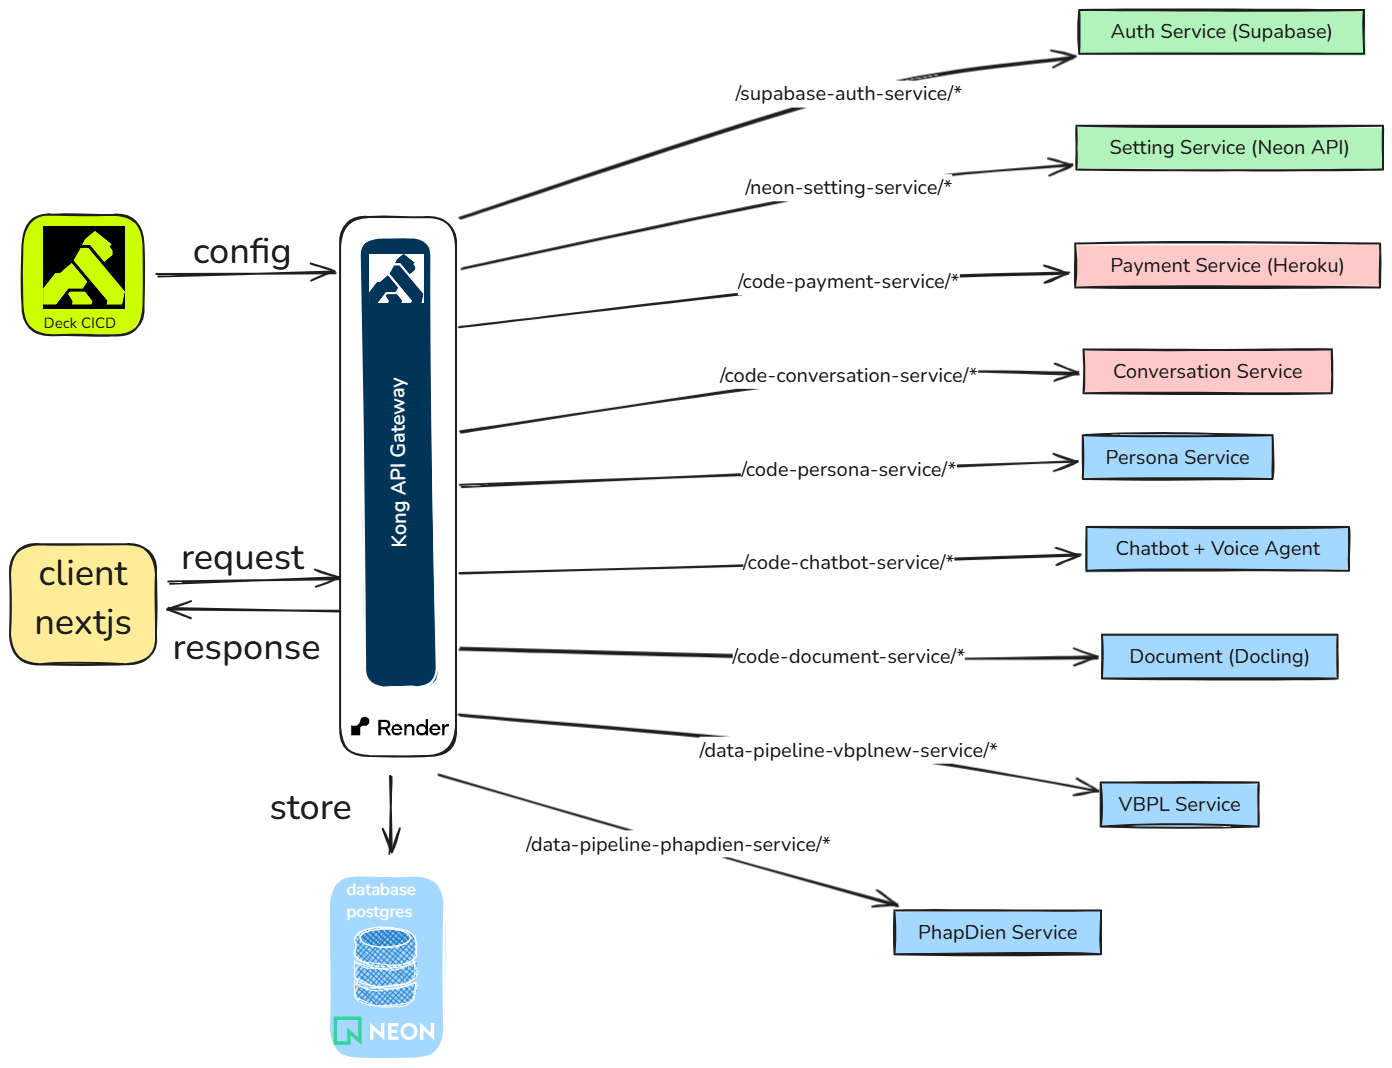
\includegraphics[width=0.95\textwidth]{pictures/request-response-result-Kong-API-Gateway.excalidraw.png}
\caption{Sơ đồ tuần tự mô tả luồng Request và Response qua Kong API Gateway}
\end{figure}

Các plugins trong dự án này:

\begin{itemize}
\item Plugin bot-detection: phân tích User-Agent và các dấu hiệu khác để chặn các request từ các bot độc hại, scraper, hoặc các công cụ tự động không mong muốn.

\item Plugin rate-limiting: giới hạn số lượng request, giúp bảo vệ các dịch vụ khỏi bị quá tải hoặc bị lạm dụng.

\item Plugin request-size-limiting: chặn các request có kích thước vượt quá ngưỡng cho phép.

\item Plugin http-log: thu thập các thông tin quan trọng về request/response và gửi qua giao thức http api NestJS và thực hiện lưu vào database postgres

\item Plugin correlation-id tạo request-id: tự động tạo ra một mã định danh duy nhất và gắn vào header của mỗi request để truy vết (tracing).

\item Plugin request-transformer thêm thông tin Request-Kong-Secret: gửi header chứa mã bí mật vào request trước khi đẩy xuống dịch vụ để các request phải được gọi từ Kong API Gateway.
\end{itemize}

\begin{figure}[H]
\centering
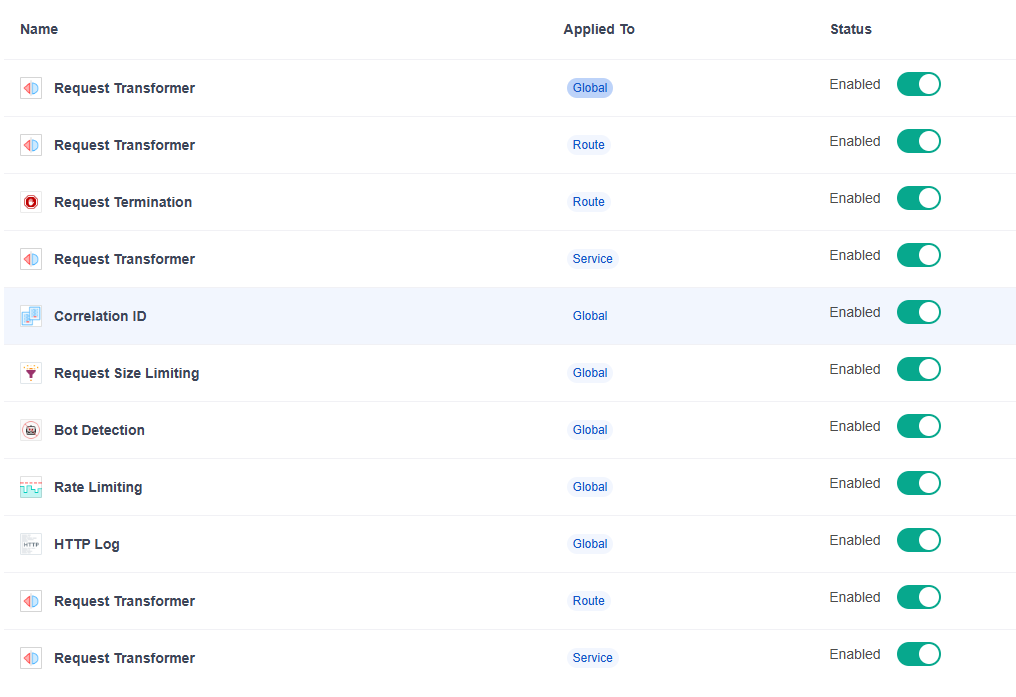
\includegraphics[width=0.95\textwidth]{pictures/kong-api-gateway-plugin.png}
\caption{Danh sách các plugin được cấu hình trên Kong API Gateway}
\end{figure}
\begin{figure}[H]
\centering
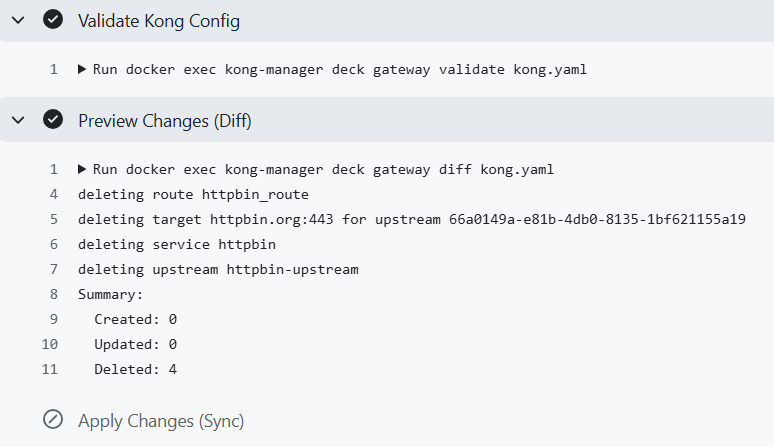
\includegraphics[width=0.95\textwidth]{pictures/kong-api-gateway-github-action-v2.png}
\caption{Luồng CI/CD triển khai cấu hình Kong API Gateway qua GitHub Actions}
\end{figure}

\begin{figure}[H]
\centering
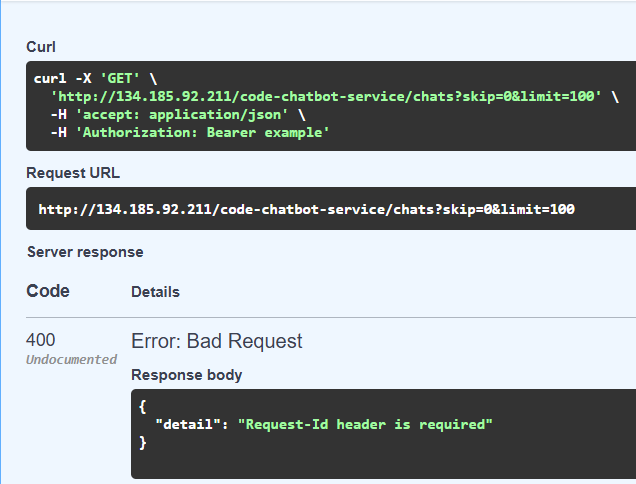
\includegraphics[width=0.95\textwidth]{pictures/kong-api-gateway-request-id-not.png}
\caption{Phản hồi lỗi từ hệ thống khi yêu cầu (Request) thiếu mã định danh Request ID}
\end{figure}

\begin{figure}[H]
\centering
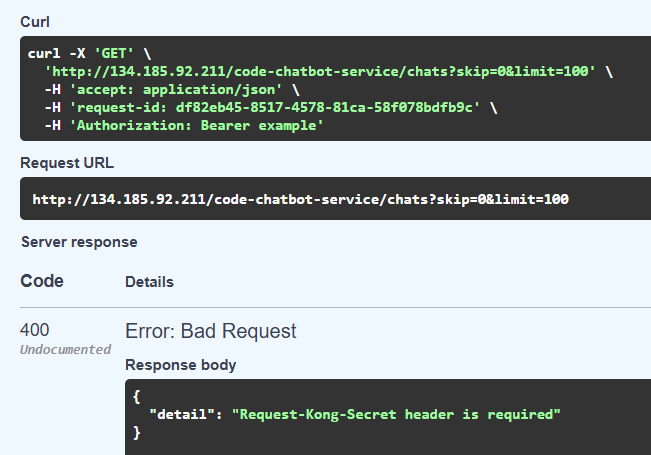
\includegraphics[width=0.95\textwidth]{pictures/kong-api-gateway-request-kong-secret-not.png}
\caption{Phản hồi chặn truy cập từ Kong API Gateway khi yêu cầu thiếu mã bảo mật Kong Secret}
\end{figure}

\begin{figure}[H]
\centering
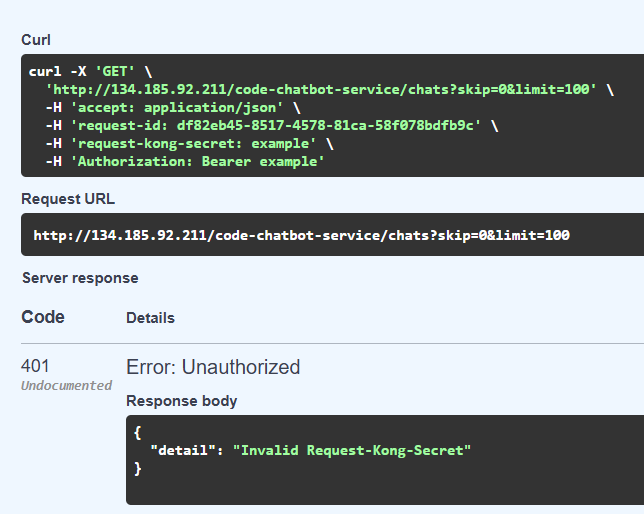
\includegraphics[width=0.95\textwidth]{pictures/kong-api-gateway-request-kong-secret-invalid.png}
\caption{Phản hồi lỗi xác thực từ Kong API Gateway khi mã bảo mật Kong Secret không hợp lệ}
\end{figure}
